%\newpage
\section{Factual}
\label{sec::Factual}
%\textbf{Factual Explainers:}
We classify the factual explainer methods broadly into two categories based on the nature of the integration of the explainability architecture with the main model as follows.

% \begin{figure*}[htbp]
%   \centering
%   \vspace{-4mm}
%   %\includegraphics[]{test3_schema.pdf}
%   \includegraphics[width= .5\textwidth]{SE_PH.png}
%   \centering
%   \caption{\small \textbf{Difference between Self-Interpretable and Post-hoc architectures}  }
%   \label{fig:SE_vs_PH}
% \end{figure*}

\begin{figure}[t]
\vspace{-4mm}
     \centering
     \begin{subfigure}[b]{0.48\textwidth}
         \centering
         \includegraphics[width=\textwidth]{submissions/Sourav2023/SE_PH.png}
         \caption{Self-Interpretable \& Post-hoc}
         \label{fig:SE_vs_PH}
     \end{subfigure}
     \hfill
     \begin{subfigure}[b]{0.5\textwidth}
         \centering
         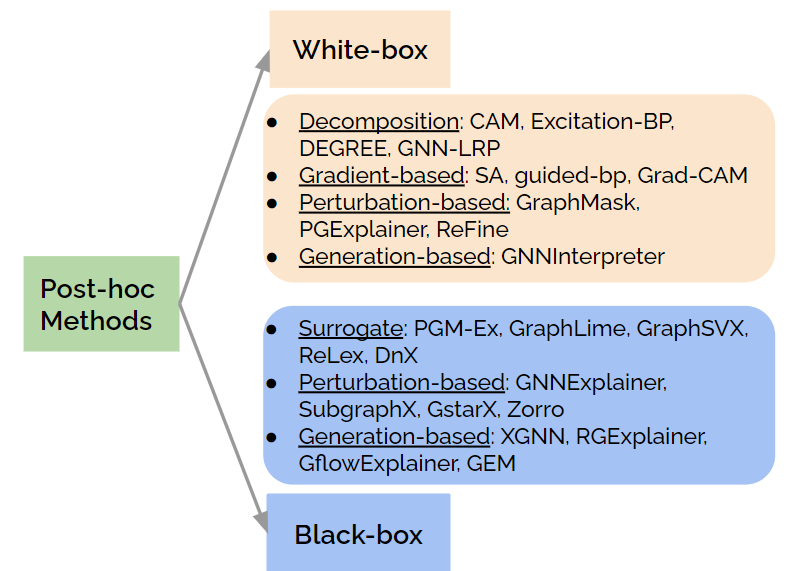
\includegraphics[width=\textwidth]{submissions/Sourav2023/white_black_box.png}
         \caption{Categorization of Post-hoc methods}
         \label{fig:white_black_box}
     \end{subfigure}
        \caption{(a) \small \textbf{Self-interpretable and post-hoc architectures :} In self-interpretable methods, the subgraph extraction module \(g\) uses constraints to find an informative subgraph \(\CG_s\) from the input graph \(\CG\). The prediction module \(f\) uses this \(\CG_s\) to predict the label \(Y\). In contrast, Post-hoc methods consider model as pre-trained with fixed weights. For any instance \(\CG\), post-hoc methods generate explanation using model's input \(\CD\), output \(Y\) and in some cases the model's internal parameters. (b) \small \textbf{White-box and Black-box 
        % Categorizing post-hoc methods as 
        post-hoc methods:} Methods are shown in the individual categories. Decomposition-based: CAM \cite{Excitation-BP}, Excitation-BP \cite{Excitation-BP}, DEGREE \cite{degree}, GNN-LRP \cite{GNN-LRP}; Gradient-based: SA \cite{guided-bp} , Guided-BP \cite{guided-bp} , Grad-CAM \cite{Excitation-BP}; Surrogate: PGM-Ex \cite{pgexplainer}, GraphLime \cite{graphlime}, GraphSVX \cite{graphsvx}, ReLex \cite{RELex}, DnX \cite{distilexplain}; Perturbation-based: GNNExplainer~\cite{ying2019gnnexplainer}, GraphMask \cite{Graph-mask}, PGExplainer \cite{pgexplainer}, ReFine \cite{ReFine}, ZORRO \cite{zorro}, SubgraphX \cite{subgraphX}, GstarX \cite{gstarx}; Generation-based: XGNN \cite{xgnn}, RGExplainer \cite{RL-enhanced}, GNNInterpreter \cite{gnninterpreter}, GFlowExplainer \cite{Gflow}, GEM \cite{Gen-causal}.}
        \label{}
\end{figure}

% The explainability architecture finds the relevant subset of the input which is used to make prediction and also acts as the explanation.

\begin{itemize}
\item \textbf{Post-hoc:} Post-hoc methods do not have the explainable architecture inbuilt into the model to attribute a model's prediction to the input. As seen in Figure \ref{fig:SE_vs_PH}, the explainability architecture (EA) is separated from the model which is pre-trained with fixed weights. For any instance \(\CG\), post-hoc methods generate an explanation using the model's input \(\CD\), output \(Y\) and sometimes even internal parameters of the model. Note that different EAs use different inputs \(\CD\) that are fed to the model. Post-hoc methods might not be always accurate as they may end up extracting features that are spuriously correlated with the task \cite{protgnn, not-posthoc, GSAT,kosan2023robust}.

\item \textbf{Self-interpretable:} Contrary to post-hoc methods, self-interpretable explainable methods design explainability architecture directly inside the model. As seen in Figure \ref{fig:SE_vs_PH}, these methods usually have two modules. The subgraph extraction module (the function \(g\)) uses constraints to find an informative subgraph \(\CG_s\) from the input graph \(\CG\). Then, the prediction module \(f\) uses \(\CG_s\) to predict label \(Y\). \(\CG_s\) also acts as an explanation. Both modules are trained together with an objective  \(L(f \circ g(\CG), Y)\) to minimize the loss between prediction \(f \circ g (\CG)\) and label $Y$. One major drawback of self-interpretable models is that the good interpretability of the models is often at the cost of the prediction accuracy \cite{GSAT}.

%Based on design of the explainability, we further classify the self-interpretable methods into two types - 1) constraint based and 2) Parameter based. If the design of the explainability architecture is based on constraints (e.g., structural) then we classify them as constraint based methods. Typically, two types of constraints are used - 1) Information constraints and 2) Structural constraint. However, if the design of explainability is based on using parameter of the model, we classify them as parameter based methods.

\end{itemize}




\subsection{Post-hoc}
\label{sec:post_hoc}
%Based on the techniques used to find explanation, we categorize these Post-hoc methods into a) Decomposition-based methods (Sec. \ref{sec:white_decom}), b) Gradient-based methods (Sec. \ref{sec::gradient-based}), c) Surrogate methods (\ref{sec::surrogate_methods}), d) Perturbation-based methods (Sec. \ref{sec::perturbation}), e) Generation-based methods (\ref{sec::generation-based}).\\
We divide the post-hoc methods based on their approaches used to find explanation into the following categories: a) Decomposition-based methods (Sec. \ref{sec:white_decom}), b) Gradient-based methods (Sec. \ref{sec::gradient-based}), c) Surrogate methods (\ref{sec::surrogate_methods}), d) Perturbation-based methods (Sec. \ref{sec::perturbation}), e) Generation-based methods (\ref{sec::generation-based}). The post-hoc methods can also be categorized based on their requirement to access the internal parameters of the model. As seen in figure \ref{fig:white_black_box}, this division results into the following categories of the methods: \textbf{white-box} and \textbf{black-box}. \\
\noindent
\textbf{White-box}: These methods require access to internal model parameters or embeddings to provide explanations. For instance, all decomposition-based methods (Sec. \ref{sec:white_decom}) require model parameters such as node weights of each layer to compute an importance score of different parts of the input. Even gradient based methods (Sec. \ref{sec::gradient-based}) require access to the gradients. Thus, all methods in these categories are considered as white-box methods and they are not suitable in cases where a model's internal parameters are inaccessible.\\
\noindent
 \textbf{Black-box}: Contrary to the white-box methods, black-box methods do not require access to the model's internal parameters. For instance, all approaches in the category of surrogate methods (Sec. \ref{sec::surrogate_methods}) generate a local dataset using the model's input and output. Since these methods do not require access to the model parameters, all of them can be categorized as black-box methods.
    % \item \textbf{Mixed} In these categories, an approach may either be white-box or black-box. For instance,  Perturbation based methods may  \cite{pgexplainer,Graph-mask} or may not access model parameters \cite{ying2019gnnexplainer}. Same is the case with generation based methods.
%\end{itemize} 

 %Note that some of the categories 
%Another way of categorizing post-hoc methods is based on whether it requires access to the internal parameters of the model. There are two kinds of method: \textbf{White-box and Black-box}. 

% \begin{figure*}[tb]
%   \centering
%   \vspace{-4mm}
%   %\includegraphics[]{test3_schema.pdf}
%   \includegraphics[width= .8\textwidth]{SE_summary.png}
%   \centering
%   \caption{\small \textbf{ Summary of Self-interpretable methods: } Every self-interpretable method has two key modules - a subgraph extraction module and a prediction module. The subgraph extraction module (the function \(g\)) uses constraints to find an informative subgraph \(\CG_s\) from input graph \(\CG\). Then, the prediction module uses \(\CG_s\) to predict label \(Y\). The figure displays technique used by each method to implement both these modules. Self-interpretable Methods are categorized as: 1) Information constraints methods: GIB \cite{GIB}, VGIB \cite{VGIB}, GSAT \cite{GSAT}, LRI \cite{inject-explain}; 2) Structure Constraints methods: DIR \cite{D_invariant_rationale}, ProtGNN \cite{protgnn}, SEGNN \cite{SE-GNN}, KER-GNN \cite{kergnns} }
  
  
%   \label{fig:SE_summary}
% \end{figure*}

  % \caption{\small \textbf{Overview of the Schema.} \textbf{(1) Factual.}  Information constraints methods: GIB \cite{GIB}, VGIB \cite{VGIB}, GSAT \cite{GSAT}, LRI \cite{inject-explain}; Structure Constraints methods: DIR \cite{D_invariant_rationale}, ProtGNN \cite{protgnn}, SEGNN \cite{SE-GNN}, KER-GNN \cite{kergnns}; Decomposition methods: CAM \cite{Excitation-BP}, Excitation-BP \cite{Excitation-BP}, DEGREE \cite{degree}, GNN-LRP \cite{GNN-LRP}; Gradient-based methods: SA \cite{guided-bp} , Guided-BP \cite{guided-bp} , Grad-CAM \cite{Excitation-BP}; Surrogate Methods: PGM-Ex \cite{pgexplainer}, GraphLime \cite{graphlime}, GraphSVX \cite{graphsvx}, ReLex \cite{RELex}, DnX \cite{distilexplain}; Perturbation based methods: GNNExplainer\cite{ying2019gnnexplainer}, GraphMask \cite{Graph-mask}, PGExplainer \cite{pgexplainer}, ReFine \cite{ReFine}, ZORRO \cite{zorro}, SubgraphX \cite{subgraphX}, GstarX \cite{gstarx}; Generation Methods: XGNN \cite{xgnn}, RGExplainer \cite{RL-enhanced}, GNNInterpreter \cite{gnninterpreter}, GFlowExplainer \cite{Gflow}, GEM \cite{Gen-causal}; \textbf{(2) Counterfactual.} Search-based methods : MMACE \cite{agnostic-counter} , MEG \cite{meg-counter}, Neural Network based: RCExplainer \cite{robust-counter}, CLEAR \cite{clear-counter}; Perturbation based methods: GREASE \cite{chen2022grease}, CF2 \cite{cf^2-counter}, CF-GNNexplainer \cite{cfgnnex}
  % }


% White-box methods require access to the internal model parameters. On the other hand, Black-box models do not access the model parameters and only utilize the input and output of the model.

%They can be classified as 1) Decomposition methods that decompose the model's prediction layer by layer and assign a importance score to input, and 2) Gradient-based methods that use gradient information of the model to provide explanation.  

%They can be categorized into 1) Surrogate methods that construct simple explainable model that fit the predictions, 2) Perturbation methods perturb the input and study its impact on output to find the important parts of input, 3) Generation  methods use generative approaches to find important subgraph patterns that explain predictions.

% \textbf{Black-box:} Black-box models do not have access to the model parameters and only utilize the input and output of the model to provide explanations. %Based on the nature of the methods, they can be categorized into the following categories. \textbf{1)Perturbation-based, (2) Surrogate, and (3) Generation-based.}\\


%\textbf{Notations.} We define some specific notations for the GNNs that have a Global Average Pooling layer (GAP) and a fully connected layer as the final classifier. Let $e_n$ be the final embedding of node $n$ just before the GGAP layer, $g$ be the vector after the GAP layer, and $w^c$ be the weight vector of the classifier for class $C$. Then $g = \frac{1}{N} \sum_{n=1}^{N} e_n$ and the final class score $y^c$ of \textit{C} can be computed as $y^c = w^Tg$.

\subsubsection{Decomposition-based Methods}
\label{sec:white_decom}

These methods consider the prediction of the model as a score that is decomposed and distributed backwards in a layer by layer fashion till it reaches the input. The score of different parts of the input can be construed as its importance to the prediction. However, the decomposition technique can vary across methods. They also require internal parameters of the model to calculate the score. Hence, these explanation methods are considered as white-box methods. Table \ref{tab::decomposition} provides a summary of these methods. %We provide key highlights of all the methods in this category in table \ref{tab::decomposition}

\begin{table}[tb]
\vspace{-2mm}
  \centering
  \scriptsize
  \caption{Key highlights of \textit{decomposition-based} methods }
    % \resizebox{\columnwidth}{!}{%
    \begin{tabular}{cccc}
    \toprule
          \textbf{Method} & \textbf{Parameters} & \textbf{Form of Explanation} & \textbf{Task}  \\  \midrule
        CAM \cite{Excitation-BP} & \makecell{Node embedding of last layer \\and MLP weights} & Node importance  & \makecell{Graph Classification}  \\  \hline
        Excitation-BP \cite{Excitation-BP} & \makecell{Weights of all GNN layers} &  Node importance & \makecell{Node and Graph Classification }  \\ \hline
        DEGREE \cite{degree} & \makecell{Decomposes messages and\\ requires all parameters} & Similar nodes & \makecell{Node and Graph Classification}  \\ \hline
        GNN-LRP \cite{GNN-LRP} & \makecell{Weights of all layers} & \makecell{Collection of edges} & \makecell{Node and Graph Classification} \\ 
        \bottomrule
    \end{tabular}%
    % }
  \label{tab::decomposition}%
\end{table}%

One of the decomposition-based methods, \textbf{CAM} \cite{Excitation-BP} aims at constructing the explanation of GNNs that have a Global Average Pooling (GAP) layer and a fully connected layer as the final classifier. Let $e_n$ be the final embedding of node $n$ just before the GAP layer and $w^c$ be the weight vector of the classifier for the class $C$. The importance score of the node $n$ is computed as $(w^c)^Te_n$. This means that the node's contribution to the class score $y^c$ is taken as the importance. It is clear that this method is restricted to GNNs that have a GAP layer and perform only the graph classification task.


Another method, \textbf{Excitation-BP} \cite{Excitation-BP} considers that the final probability of the prediction can be decomposed into excitations from different neurons. The output of a neuron can be intuitively understood as the weighted sum of excitations from the connected neurons in the previous layer combined with a non-linear function where the weights are the usual neural network parameters. With this, the output probability can be distributed to the neurons in the previous layer according to  the ratios of these weights. Finally, the importance of a node is obtained by combining the excitations of all the feature maps of that node.

Contrary to other methods, \textbf{DEGREE} \cite{degree} finds explanation in the form of subgraph structures. First, it decomposes the message passing feed-forward propagation mechanism of the GNN to find a contribution score of a group of target nodes. Next, it uses an agglomeration algorithm that greedily finds the most influential subgraph as the explanation. \textbf{GNN-LRP} \cite{GNN-LRP} is based on the concept that the function modeled by GNN is a polynomial function in the vicinity of a specific input. The prediction score is decomposed by approximating the higher order Taylor expansion using layer-wise relevance propagation \cite{LRP-main}. This differs from other decomposition-based methods not only in the decomposition technique but also in the score attribution. While other methods attribute scores to nodes or edges, GNN-LRP attributes scores to walks i.e., a collection of edges. 



%The methods in this category consider prediction of the model as a score that is decomposed and distributed backwards layer by layer till it reaches the input. The score of different parts of the input can be construed as its importance to the prediction. The decomposition technique vary across methods. All techniques require internal parameters of the model to calculate score. Hence the explanation methods in this category are considered as white-box methods.

%\textbf{CAM} \cite{Excitation-BP} aims at the explanation of GNNs that have a Global Average Pooling layer (GAP) and a fully connected layer as the final classifier. Following the notations defined in \textbf{4.2}, the importance score of the node $n$ is computed as $(w^c)^Te_n$. This mean the node's contribution to the class score $y^c$ is taken as the importance. It is clear that this method is restricted to GNNs that have a GAP layer and perform graph classification task.\\
%\textbf{Excitation-BP} \cite{Excitation-BP} In this method, we consider that the final probability of the prediction can be decomposed into excitations from different neurons. Since the excitation of a neuron can be intuitively understood as the weighted sum of excitations from the connected neurons in previous layer, using the same weights we can attribute the excitation of neuron to previous layers. Finally, we sum up the excitations of all the feature maps of a node to get it's importance\\
%\textbf{DEGREE} \cite{degree} Contrary to other methods, DEGREE finds explanation in the form of subgraph structure. First, it decomposes the message passing feed-forward propogation mechanism of GNN to find a contribution score of target node groups. Then, it uses an agglomeration algorithm that greedily finds the most influential subgraph that is used as explanation.\\
%\textbf{GNN-LRP: } \cite{GNN-LRP} The method is based on the concept that the function implemented by GNN is locally polynomial with the input graph. The prediction score is decomposed by approximating the higher order Taylor expansion using Layer-wise relevance propogation \cite{LRP-main}. This method differs from other decomposition methods not only in decomposition technique but also in score attribution. While other methods attribute score to nodes or edges, GNN-LRP attributes the score to walks i.e. collection of edges. \\

\subsubsection{Gradient-based Methods}
\label{sec::gradient-based}
The gradient-based explainer methods follow the following key idea. Gradients represent the rate of change, and the gradient of the prediction with respect to the input represents how sensitive the prediction is to the input. This sensitivity is seen as a measure of importance. We provide a summary of these methods in Table \ref{tab::wb-gradient}.

\textbf{Sensitivity Analysis (SA)} \cite{guided-bp} is one of the earlier methods to use gradients to explain GNNs. Let $x$ be an input, which can be a node or an edge feature vector, $SA(x)$ be its importance, and $\phi$ be the GNN model, then the importance is computed as $SA(x) \propto ||\nabla_{x} \phi(x)||^{2}$. The intuition behind this method is based on the aforementioned sensitivity to the input. \textbf{Guided Backpropagation (Guided-BP)} \cite{guided-bp}, a slightly modified version of the previous method SA, follows a similar idea except the fact that the negative gradients are clipped to zero during the backpropagation. This is done to preserve only inputs that have an excitatory effect on the output. Intuitively, since positive and negative gradients have opposing effect on the output, using both of them could result in less accurate explanations.

%\textbf{Sensitivity Analysis (SA)} \cite{guided-bp} is one of the first methods to use gradients to explain a GNN's prediction. Let $x$ be an input, which can be a node or an edge feature vector, and $SA(x)$ is it's importance, and $\phi$ be the GNN, then the importance is computed as $SA(x) \propto ||\nabla_{x} \phi(x)||^{2}$. The intuition behind this method based on the aforementioned sensitivity to the input. \textbf{Guided Backpropagation (Guided-BP)} \cite{guided-bp}, a slightly modified version of the previous method, follows similar idea except the negative gradients are clipped to zero during backpropagation. This is done to preserve only inputs that have an excitatory effect on the output. An intuitive reasoning for this could be, since positive and negative gradients have opposing effect on the output, using them both could result in incorrect explanations.

The method \textbf{Grad-CAM} \cite{Excitation-BP} builds upon \textbf{CAM} \cite{Excitation-BP} (see Section \ref{sec:white_decom}), and uses gradients with respect to the final node embeddings to compute the importance scores.  The importance score is $(\frac{1}{N}\sum_{n=1}^{N}\nabla_{e_n}(y^c))^Te_n$, where $e_n$ is the final embedding of node $n$ just before the GAP layer, and $w^c$ is the weight vector of the classifier for class $C$, $g = \frac{1}{N} \sum_{n=1}^{N} e_n$ is the vector after the GAP layer, and the final class score $y^c$ of \textit{C} is $w^Tg$.
This removes the restriction about the necessity of GAP layer. This equation shows that the importance of each node is computed as the weighted sum of the feature maps of the node embeddings, where the weights are the gradients of the output with respect to the feature maps.

All the above methods depend on this particular intuition that the gradients can be good indicators of importance. However, this might not be useful in many settings. Gradients indicates sensitivity which does not reflect importance accurately. Moreover, saturation regions where the prediction of the model does not change significantly with the input, can be seen as another issue in SA and Guided-BP.

\begin{table}[tb]
  \centering
  \vspace{-2mm}
  \scriptsize
  \caption{Key highlights of \textit{gradient-based} methods}
  \resizebox{\columnwidth}{!}{%
    \begin{tabular}{ccccc}
    \toprule
        \textbf{Method} & \textbf{Explanation Type} & \textbf{Task} & \textbf{Explanation Target} & \textbf{Datasets Evaluated}  \\  \midrule
        SA \cite{guided-bp} & Instance level & \makecell{Graph classification\\Node classification} & \makecell{Nodes, Node features\\Edges, Edge features} & \makecell{Infection, ESOL \cite{esol}} \\  \hline
        Guided-BP \cite{guided-bp} & Instance level & \makecell{Graph classification\\Node classification} & \makecell{Nodes, Node features\\Edges, Edge features} & \makecell{Infection, ESOL \cite{esol}} \\  \hline
        Grad-CAM \cite{Excitation-BP} & Instance level & \makecell{Node classification} & \makecell{Nodes, Node features} & \makecell{BBBP, BACE, TOX21 \cite{kersting2016benchmark}} \\ 
    \bottomrule
    \end{tabular}}
  \label{tab::wb-gradient}%
\end{table}%

%Let $e_n$ be the final embedding of node $n$ just before the GGAP layer, $g$ be the vector after the GAP layer, and $w^c$ be the weight vector of the classifier for class $C$. Then $g = \frac{1}{N} \sum_{n=1}^{N} e_n$ and the final class score $y^c$ of \textit{C} can be computed as $y^c = w^Tg$.


%and uses gradients with respect to final node embeddings to compute the importance score. Following the notations defined in \textbf{4.2}, we compute the importance score as $(\frac{1}{N}\sum_{n=1}^{N}\nabla_{e_n}(y^c))^Te_n$. This removes the restriction about the necessity of GAP layer. This equation shows that the importance of each node is computed as the weighted sum of the node embedding's feature maps(embedding vector's components), where the weights are the gradients of the output with respect to the feature maps.

%All the above methods depend on the heuristic that gradients are a good indicator of importance. However, this is just a heuristic and not necessarily true in all settings. Gradients reflect sensitivity, however that doesn't reflect importance accurately. Saturation regions where the prediction of the model does not change significantly with the change in the input, can be seen as another issue in SA and Guided-BP.


%Another issue with these methods, especially \textbf{SA} and \textbf{Guided-BP}, is saturation regions of the model, where the model's prediction doesn't change significantly with the input \cite{sst-datasets}.



%that construct simple explainable model that fit the predictions, 2) Perturbation methods perturb the input and study its impact on output to find the important parts of input, 3) Generation  methods use generative approaches to find important subgraph patterns that explain predictions.


\subsubsection{Surrogate Methods}
\label{sec::surrogate_methods}
 Within a large range of input values, the relationship between input and output can be complex. Hence, we need complex functions to model this relationship and the corresponding model might not be interpretable. However, in a smaller range of input values, the relationship between input and output can be approximated by simpler and interpretable functions. This intuition leads to \textit{surrogate methods} that fit a simple and interpretable surrogate model in the locality of the prediction. Table \ref{tab::surrogate} shows different locality-based data extraction techniques and surrogate models used by surrogate methods. This surrogate model can then be used to generate explanations. As seen in the figure \ref{fig:Surrogate_schema}, these methods adopt a two-step approach. Given an instance \(\CG\), they first generate data from the prediction's neighborhood by utilizing multiple inputs  \(D\) within the vicinity and recording the model's prediction \(Y\). Subsequently, a surrogate model is employed to train on this data. The explanation \(E\) provided by the surrogate model serves as an explanation for the original prediction.  
%  \begin{figure*}[htbp]
%   \centering
%   \vspace{-4mm}
%   %\includegraphics[]{test3_schema.pdf}
%   \includegraphics[width= .45\textwidth]{surrogate_method.png}
%   \centering
%   \caption{\small \textbf{Generic Schema of Surrogate Methods}  }
%   \label{fig:Surrogate_schema}
% \end{figure*}

\begin{figure}[htbp]
\vspace{-2mm}
     \centering
     \begin{subfigure}[b]{0.43\textwidth}
         \centering
         \includegraphics[width=\textwidth]{submissions/Sourav2023/surrogate_method.png}
         \caption{\textbf{Generic schema of surrogate methods}}
         \label{fig:Surrogate_schema}
     \end{subfigure}
     \hfill
     \begin{subfigure}[b]{0.54\textwidth}
         \centering
         \includegraphics[width=\textwidth]{submissions/Sourav2023/perturbation_method.png}
         \caption{\textbf{Generic schema of perturbation-based methods}}
         \label{fig:Perturbation_schema}
     \end{subfigure}
        \caption{\small \textbf{a) Surrogate:} These methods follow a two-step process. For any instance \(\CG\), they generate data from the neighbourhood of the prediction by using multiple inputs \(D\) in the locality and recording its model prediction \(Y\). Then a surrogate model is used to fit this data. Explanation \(E\) for the surrogate model is the explanation for the prediction, \textbf{b) Perturbation-based:} They have two key modules: a subgraph extraction architecture and a scoring function. For an input \(G\), the subgraph extraction module extracts a subgraph \(G_s\). The model prediction \(Y_s\) for subgraph \(G_s\) are scored against the actual predictions \(Y\) using a scoring function. The feedback from the scoring function can be used to train the subgraph extraction module. Sometimes model parameters are also used as the training input to the subgraph extraction module. The optimal subgraph \(G_s^*\) acts as the final explanation \(E\). }
        \label{fig:surr_per}
\end{figure}

\textbf{PGMExplainer} constructs a Bayesian network to explain the prediction. First, it creates a tabular dataset by random perturbations on node features of multiple nodes of the computational graph and records its influence on the prediction. A grow-shrink algorithm is used to select top influential nodes. Using structure learning, a Bayesian network is learnt that optimizes the Bayesian Information Criterion (BIC) scores and the DAG of conditional probabilities act as an explanation. In \textbf{GraphLime} \cite{graphlime}, the local explanations are based on Hilbert-Schmidt Independence Criterion Lasso (HSIC Lasso) model, which is a kernel-based nonlinear interpretable feature selection algorithm. This method assumes that the node features in the original graph are easily interpretable. The HSIC model takes a node and its N-hop neighbourhood (for some $N$), and selects a subset of node features that are the most influential to the prediction. These selected features act as the explanation. To construct a local dataset, \textbf{GraphSVX} \cite{graphsvx} uses a mask generator to jointly perturb the nodes and the features and observes its effects on the predictions. The mask generator isolates the masked nodes and replaces masked features by its expected values. It then fits a weighted linear regression model (WLR) on the local dataset. The coefficients of WLR act as explanations.

The next two approaches use GNN based models to act as surrogate models. \textbf{RelEx} \cite{RELex} uses a BFS-based sampling strategy to select nodes and then perturb them to create the local dataset. Then, a GCN model with residual connections is used to fit this dataset. In contrast to other methods in this category, the surrogate model of RelEx is not interpretable. Hence, it uses perturbation-based strategy to find a mask that acts as explanation. We note that the surrogate model is more complex compared to other methods and it requires the use of another explanation method to derive explanations from the surrogate model. \textbf{DistilnExplain (DnX)}~\cite{distilexplain} first learns a surrogate GNN via knowledge distillation and then provides an explanation by solving a simple convex program. In contrast to RelEx, DnX uses a simpler surrogate model which is a linear architecture termed as Simplified Graph convolution (SGC) \cite{Simple-GCN}. SGC does not have any non-linear activation layers and uses a single parameter matrix across layers. The parameters in SGC are learned via knowledge distillation with an objective to minimize the KL-divergence between the predictions by SGC and the model. Furthermore, explanations can be derived from SGC by solving a simple convex program.



%The main idea of the methods in this category is to fit a simple and interpretable surrogate model in the locality of the prediction. This surrogate model can then be used to generate explanations. These methods generally follow a two steps process. First  they generate dataset from the neighbourhood of the prediction. Then, they fit a surrogate model to this dataset. Explanation of the surrogate model is considered as explanation for the prediction. \\


%\textbf{PGMExplainer} \cite{pgm-ex} The key idea is to construct a Bayesian network to explain the prediction. First, a tabular dataset is created by random perturbation of node features of multiple nodes of the computational graph and recording its influence on prediction. A grow-shrink algorithm is used to select top influential nodes. Using structure learning, a Bayesian network is learnt that optimizes BIC scores. The DAG of conditional probabilities act as explanation. \\

%\textbf{GraphLime} \cite{graphlime} In this method, the local explanations are based on Hilbert-Schmidt Independence Criterion Lasso (HSIC Lasso) model, which is a kernel based nonlinear interpretable feature selection algorithm. This method assumes that the node features in the original graph are easily interpretable. The HSIC model takes a node and it's N-hop neighbourhood(for some $N$), and selects a subset of node features (using HSIC weights) that are the most influential to the prediction, which acts as the explanation.\\

%\textbf{RelEx} \cite{RELex} It uses a bfs-based sampling strategy to select nodes and then perturb them to creates the local dataset. Then, a GCN model with residual connections is used to fit this dataset. In contrast to other methods in this category, the surrogate model of RelEx is not interpretable. Hence, it uses perturbation-based strategy to find a mask that acts as explanation. We note that the surrogate model is more complex compared to other methods and it requires use of another explanation method to derive explanation from the surrogate model. \\

%\textbf{DistilnExplain} \cite{distilexplain} DnX first learns a surrogate GNN via knowledge distillation and then provides explanation by solving a simple convex program. In contrast to RelEx, DnX uses a simpler surrogate model which a linear architecture termed as Simplified Graph convolution (SGC) \cite{Simple-GCN}. SGC does not have any non-linear activation layers and uses single parameter matrix across layers. SGC's parameters are learned via knowledge distillation with an objective to minimmize KL-divergence between SGC's and model's prediction. Explanation can then be derived from SGC by solving a simple convex program.\\

%\textbf{GraphSVX} \cite{graphsvx} To construct a local dataset, GraphSVX uses a mask genertor to jointly perturbs the nodes and the features and observes its effects on the predictions. The mask generator isolates the masked nodes and replaces masked features by its expected values. It then fits a weighted linear regression model (WLR) on the local dataset. The coefficients of WLR act as explanations.\\

\begin{table}[tb]
  \centering
  \caption{Key highlights of \textit{surrogate methods} }
    \resizebox{\columnwidth}{!}{%
    \begin{tabular}{ccccc}
    \toprule
          \textbf{Method} & \textbf{Local Dataset extraction} & \textbf{Surrogate model} & \textbf{Explanation} & \\  \midrule
        GraphLime \cite{graphlime} & N-hop neighbor nodes & HSIC Lasso  & Weights of the model & \\  
        PGMExplainer \cite{pgm-ex} & Random node feature perturbation  & Bayesian network  & DAG of conditional dependence & \\  
        ReLex \cite{RELex} & Random sampling of connected subgraphs & GCN & Perturbation-based method  &\\ 
        DistilnExplain \cite{distilexplain} & Entire dataset  & Knowledge distilled Simple GCN \cite{Simple-GCN}  & Convex programming, decomposition&  \\ 
        GraphSVX \cite{graphsvx} & Input perturbations via mask generator  & Weighted Linear Regression (WLR)   & Weights of WLR &  \\ \bottomrule
        
    \end{tabular}%
    }
  \label{tab::surrogate}%
\end{table}%













 \subsubsection{Perturbation-based Methods} 
 \label{sec::perturbation}
 These methods find \textit{important subgraphs} as explanations by perturbing the input. Fig. \ref{fig:Perturbation_schema} presents two key modules of these methods: the subgraph extraction module and the scoring function module. For an input \(G\), the subgraph extraction module extracts a subgraph \(G_s\). The model predictions \(Y_s\) for subgraphs are scored against the actual predictions \(Y\) using a scoring function. The feedback from the scoring function can be used to train the subgraph extraction module. In some cases, model parameters are also used as the training input for the subgraph extraction module. These methods provide explanations \(E\) in the form of a subgraph structure and some also provide node features as explanations. Table \ref{tab::perturbation} presents a summary of these methods.

%  \begin{figure*}[htbp]
%   \centering
%   \vspace{-4mm}
%   %\includegraphics[]{test3_schema.pdf}
%   \includegraphics[width= .5\textwidth]{perturbation_method.png}
%   \centering
%   \caption{\small \textbf{Generic Schema of Perturbation Methods}  }
%   \label{fig:Perturbation_schema}
% \end{figure*}

\textbf{GNNExplainer} \cite{ying2019gnnexplainer} is one of the initial efforts towards the explainability of GNNs. It identifies an explanation in the form of a Subgraph including a subset of node features that have the maximum influence on the prediction. It learns continuous masks for both adjacency matrix and features by optimizing cross entropy between the class label and model prediction on the masked subgraph. In
 a follow-up work, \textbf{PGExplainer} \cite{pgexplainer} extends the idea in GNNExplainer by assuming the graph to be a random Gilbert graph, where the probability distribution of edges is conditionally independent. The distribution of each edge is independently modeled as a Bernoulli distribution, i.e., each edge has a different parametric distribution. These parameters are modeled by a neural network (MLP), and the parameters of this MLP is computed by optimizing the mutual information between the explanation subgraph and the predictions of the underlying GNN model. Another masking-related method, \textbf{GraphMask} \cite{Graph-mask} provides an explanation by learning a parameterized edge mask that predicts the edge to drop at every layer. A single-layer MLP classifier is trained to predict the edges that can be dropped. To keep the topology unaffected, these edges are not dropped but are replaced by a learned baseline vector. The training objective is to minimize the $L_0$ norm i.e., the total number of edges not masked, such that the prediction output remains within a tolerance level. To make the objective differentiable, it uses sparse relaxations through the reparameterization trick and the hard concrete distribution \cite{concrete-distri, repara-trick}. 
 
 Another approach \textbf{Zorro} \cite{zorro} finds explanations in the form of important nodes and features that maximizes \textit{Fidelity} (see Sec. \ref{sec::eval}). It uses a greedy approach that selects the node and the feature at each step with the highest fidelity score. Fidelity is computed as the expected validity of the perturbed input. The approach uses a discrete mask for selecting a subgraph without any backpropagation.
A two-staged approach, \textbf{ReFine} \cite{ReFine} consists of the edge attribution or pre-training and the edge selection or fine-tuning steps. During pre-training, a GNN and an MLP are trained to find the edge probabilities for the entire class by maximizing mutual information and contrastive loss between classes. During the fine-tuning step, the edge probabilities from the previous stage are used to sample edges and find an explanation that maximizes mutual information for a specific instance.

The next two approaches use cooperative game theoretic techniques. \textbf{SubgraphX} \cite{subgraphX} applies the Monte Carlo Tree search technique for subgraph exploration and uses the Shapley value \cite{Shap_val} to measure the importance of the subgraphs. For the search algorithm, the child nodes are obtained by pruning the parent graph. In computing the Shapley values, the Monte Carlo sampling helps to find a coalition set and the prediction from the GNN is used as the pay-off in the game. In a subsequent work, \textbf{GStarX} \cite{gstarx} uses a different technique from cooperative game theory known as HN value \cite{HN-val}, to compute importance scores of a node for both graph and node classification tasks. In contrast to the Shapley value, the HN value is a structure-aware metric. Since computing the HN values is expensive, Monte Carlo sampling is used for large graphs. The nodes with the top-k highest HN values act as an explanation.
 
 % black box explanation
 
%\textbf{GNNExplainer} \cite{ying2019gnnexplainer} is one of the initial efforts in explainability of GNNs. It identifies a subgraph and subset of node features that influence predictions as explanation. It learns continuous masks for both adjacency matrix and features by optimzing cross entropy between the label class and model prediction on masked subgraph.\\
%\textbf{SubgraphX} \cite{subgraphX}  The key idea of this method is to use monte-carlo tree search for subgraph exploration and use shapley value to measure subgraph importance. For search algorithm, the child nodes are obtained by pruning the parent graph. To calculate Shapley value, monte-carlo sampling is used to find a coalition set and GNN's prediction is used as game-gain.\\ % black box explanation
%\textbf{PGExplainer} \cite{pgexplainer}  This method extends the idea in \textbf{GNNExplainer} \cite{ying2019gnnexplainer} by assuming the graph to be a random Gilbert graph, where the probability distribution of edges are conditionally independent. The distribution of each edge is independently modelled as a Bernoulli distribution, i.e., each edge has different parameteric distribution. These parameters are modelled by a neural network(MLP), and the parameters of this MLP is computed by optimizing mutual information between explanation subgraph and the GNN's predictions. \\ % jaspal
%\textbf{GraphMask} \cite{Graph-mask}. This method provides explanation by learning a parameterized edge mask that predicts which edge to drop at every layer. A single layer MLP classifier is trained to predict the edges that can be replaced by a learned baseline. The training objective is to minimize L0 norm i.e. total number of edges not masked such that prediction output remains within a tolerance level. To make the objective differentiable, it uses sparse relaxation through hard concrete distribution and reparameterization trick.\\ %its a white box approach - uses hidden layer information for edge importance prediction
%\textbf{Zorro} \cite{zorro} It finds explanation in the form of important nodes and features that maximizes Fidelity. It uses a greedy combinatorial approach that selects the node and feature at each step with highest fidelity score. Fidelity is computed as expected validity of noise perturbed input. The approach uses discrete mask for selecting subgraph as there is no backpropogation involved.\\
%\textbf{ReFine} \cite{ReFine} The approach consists of two stages edge attribution or pre-training and edge selection or fine-tuning. During pre-training, a GNN and MLP is trained to find edge probabilities for the entire class by maximizing mutual information and contrastive loss between classes. During fine-tuning, the edges probabilities from previous stage is used to sample edges and find explanation that maximizes mutual information for a specific instance.\\
%The next two approaches use co-operative game theoretic techniques. \textbf{SubgraphX} \cite{subgraphX} uses monte-carlo tree search for subgraph exploration and use shapley value to measure subgraph importance. For search algorithm, the child nodes are obtained by pruning the parent graph. To calculate Shapley value, monte-carlo sampling is used to find a coalition set and GNN's prediction is used as game-gain.

%\textbf{GStarX: } \cite{gstarx} Inspired by co-operative game theory, this approach uses HN-value to compute importance scores of a node for graph and node classification tasks. In contrast to Shapley value, HN-value is structure aware metric. Since HN value calculation is computationally expensive, monte carlo sampling is used for larger graphs. Top k highest HN-value nodes act as explanation.\\ \\

% can add: Node features used/not used ; White-box/back-box
\begin{table}[tb]
\vspace{-2mm}
  \centering
  \caption{Key highlights of the \textit{perturbation-based} methods.}
    \resizebox{\columnwidth}{!}{%
    \begin{tabular}{ccccc}
    \toprule
          \textbf{Method} & \textbf{Subgraph Extraction Strategy} & \textbf{Scoring function} & \textbf{Constraints} & \textbf{Node Feature Explanation}  \\  \midrule
        GNNExplainer \cite{ying2019gnnexplainer} & Continuous relaxation  & Mutual Information  & Size  & Yes  \\  
        SubgraphX \cite{subgraphX} & Monte Carlo Tree Search & Shapley Value  & Size, connectivity  & No \\  
        GraphMask \cite{Graph-mask} & Layer-wise parameterized edge selection &  $L_0$ norm  & Prediction divergence & No \\  
        PGexplainer \cite{pgexplainer} & Parameterized edge selection & Mutual Information & Size and/or connectivity & No \\  
        Zorro \cite{zorro} & Greedy selection & Fidelity & Threshold fidelity & Yes  \\  
        ReFine \cite{ReFine} & Parameterized edge attribution & Mutual Information  & Number of edges  & No \\  
         GstarX \cite{gstarx} & Monte Carlo sampling & HN-value  & Size  & No  \\  \bottomrule
    \end{tabular}%
    }
  \label{tab::perturbation}%
\end{table}%


\begin{table}[tb]
  \centering
  \scriptsize
  \caption{Key highlights of the \textit{generation-based} methods }
    \begin{tabular}{ccccc}
    \toprule
          \textbf{Methods} & \textbf{Explanation Type} & \textbf{Optimization} & \textbf{Constraints} & \textbf{Task}  \\  \midrule
        XGNN \cite{xgnn} & Model level & RL-policy gradient  & Domain specific rules  & Graph classification  \\  
        RG-Explainer \cite{RL-enhanced} & Instance level & RL-policy gradient  & Size, radius, similarity & Node \& Graph classification \\  
        GFLOW Explainer \cite{Gflow} & Instance level & TD flow matching  & Connectivity / cut vertex  & Node \& Graph classification \\  
        GNNinterpreter \cite{gnninterpreter} & Model level & Continuous relaxation  & Similarity to mean & Graph Classification \\  
        GEM \cite{Gen-causal}& Instance level & Autoencoder  & Graph validity rules  & Node \& Graph Classification \\  
        \bottomrule
    \end{tabular}%
  \label{tab::generation}%
\end{table}%

 
\subsubsection{Generation-based methods}
\label{sec::generation-based}
Generation-based approaches either use generative models or graph generators to derive instance-level or model-level explanations.
Furthermore, to ensure the validity of the generated graphs, different approaches have been proposed. Table \ref{tab::generation} provides a summary of the generation-based methods.    %\\

%Approaches in this category use some form of graph generators. 
\textbf{XGNN}~\cite{xgnn} provides model-level explanations by generating key subgraph patterns to maximize prediction for a certain class. The subgraph is generated using a Reinforcement learning (RL) based graph generator which is optimized using policy gradient. In the setup for the RL agent, the previous graph is the state; adding an edge is an action; and the model prediction along with the validity rules acts as the reward. Unsurprisingly, the validity rules are specified based on domain knowledge.  Another RL-based method, \textbf{RG-Explainer} \cite{RL-enhanced} formulates the underlying problem as combinatorial optimization instead of using continuous relaxation or search methods to find the subgraph. A starting point is selected using an MLP which acts as an input to the graph generator. The graph generator is an RL agent that optimizes for the policy using policy gradient with subgraph as the state, adding neighboring nodes as the action, and the function of the cross entropy loss as the reward. 

A non-RL method, \textbf{GNNinterpreter} \cite{gnninterpreter} is a generative model-level explanation method for the graph classification task. Its objective is to maximize the likelihood of predicting the explanation graph correctly for a given class. The similarity between the explanation graph embedding and the mean embedding of all graphs act as an optimization constraint. Intuitively, this ensures that the explanation graph stays closer to the domain and is meaningful. Since the adjacency matrix and sometimes even the features can be categorical, GNNinterpreter uses the Grumbel softmax method \cite{repara-trick} to enable backpropagation of gradients. Contrary to XGNN with domain-specific hand-crafted rules, GNNinterpreter uses numerical optimization and does not need any domain knowledge.

\textbf{GFLOW Explainer} \cite{Gflow} uses GFLOWNETs as the generative component. The objective is to construct a TD-like flow matching condition \cite{bengio-gflownet} to learn a policy to generate a subgraph by sequentially adding neighbors (nodes) such that the probability of the subgraph of a class is proportional to the mutual information between the label and the distribution of possible subgraphs. A \textit{state} consists of several nodes with the initial state as the single most influential node and the end state that satisfies the stopping criteria. \textit{Action} is adding a node and the \textit{reward} is a function of the cross-entropy loss.
%\\\\ %not a black-box approach as it needs mean embedding

 %\textbf{XGNN:}  \cite{xgnn} It provides model level explanations by generating key subgraph patterns the maximize prediction for a certain class. The subgraph is generated using a Reinforcement learning based graph generator which is optimized using policy gradient. For the RL agent, the previous graph is the state, adding and edge is an action and Model prediction along with validity rules act as reward. The validity rules are specified based on domain knowledge. \\\\
 %\textbf{RG-Explainer} \cite{RL-enhanced} Instead of using continous relaxtion or search methods to find the subgraph, RG-explainer formulates the combinatorial optimization as Reinforcement learning problem. A starting point is selected using an MLP which acts as an input to the graph generator. The graph generator is an RL agent optimized using policy gradient with sugraph as state, adding neighbouring nodes as action and cross entropy loss as reward.  \\\\
 %\textbf{GNNinterpreter:} \cite{gnninterpreter} It is a generative model level explanation method for graph classification task. The objective is to find a graph that maximizes the scoring function before softmax for a class. The optimization is constraint by similarity of mean embeddings so that explanation is meaningful. Since the adjacency matrix and sometimes even the features can be categorical, GNNinterpreter uses Grumbel softmax trick to enable backpropogation of gradients. Contrary to XGNN that uses Reinforcement learning and uses domain specific hand-crafted rules, GNN interpreter uses numerical optimization and does not need any domain knowledge.\\\\ %not a black-box approach as it needs mean embedding
 %\textbf{GFLOW Explainer} \cite{Gflow} It uses GFLOWNETs as the generative component. The objective is construct a TD-like flow matching condition to learn a policy to generate a subgraph by sequentially adding neighbour node such that the probability of subgraph of a class is proportional to the mutual information. A State consists of several nodes with initial state as single most influential node and end state that satisfies stopping criteria. Action is adding a node and reward is a cross entropy function. \\\\

% \textbf{Neigborhood Generator: } The objective of this approach is to find model level the neighborhood explanation of the node that maximizes the model's prediction for that node. It uses policy gradient

% \textbf{GAN Explainer:} - Should we include this too? its on arxvix only
 
 \textbf{GEM~\cite{Gen-causal}} uses the principles of Granger causality to generate ground-truth explanations which are used to train the explainer. It quantifies the causal contribution of each edge in the computational graph by the difference in the loss of the model with and without the edge. This distilled ground-truth for the computation graph is used to train the generative auto-encoder based explainer. This explainer provides an explanation for any instance in the form of the subgraph of the computation graph.
 
 
 %\\ %sourav: Isn't GEM counterfactual?

 %\textbf{GraphEx: } \cite{graphex}  - Not including this paper. Its a Tiny paper with not much experimentation. It assumes a categorical distribution for both nodes and edges for a given class of graphs. It then solves and MLE to fit the distribution to a class (like Naive bayes).
 
 % table - model level/ instance , Task , Optimization, State, Action, Reward, Constraints (to get valid graph)
 
 
 

%%%%%%%%%% ADDING SELF INTERPRETABLE

\subsection{Self-interpretable} 
In self-interpretable methods, the explainable procedure is intrinsic to the model. Such methods derive explainability by incorporating interpretability constraints. These methods use either information constraints or cardinality (structural) constraints to derive an informative subgraph which is used for both the prediction and the explanation. Based on the design of the explainability, we further classify the self-interpretable methods into two types based on the imposed constraints (Fig. \ref{fig:SE_summary}). 
% \begin{figure*}[htbp]
%   \centering
%   \vspace{-4mm}
%   %\includegraphics[]{test3_schema.pdf}
%   \includegraphics[width= .6\textwidth]{SE_summary.png}
%   \centering
%   \caption{\small \textbf{Highlight of Self-Interpretable methods}  }
%   \label{fig:SE_summary}
% \end{figure*}

\begin{figure*}[t]
  \centering
  \vspace{-5mm}
  %\includegraphics[]{test3_schema.pdf}
  \includegraphics[width= .8\textwidth]{submissions/Sourav2023/SE_summary.png}
  \centering
  \vspace{-1mm}
  \caption{\small \textbf{Self-interpretable methods: } Every self-interpretable method has a \textit{subgraph extraction} and a \textit{prediction} module. The subgraph extraction module (the function \(g\)) uses constraints to find an informative subgraph \(\CG_s\) from input graph \(\CG\). The prediction module uses \(\CG_s\) to predict label \(Y\). This also shows the techniques used by each method to implement these individual modules. Self-interpretable Methods are categorized based on constraints: \textbf{(1) Information constraint:} GIB \cite{GIB}, VGIB \cite{VGIB}, GSAT \cite{GSAT}, LRI \cite{inject-explain}; \textbf{(2) Structural constraint:} DIR \cite{D_invariant_rationale}, ProtGNN \cite{protgnn}, SEGNN \cite{SE-GNN}, KER-GNN \cite{kergnns}.}
  
  
  \label{fig:SE_summary}
\end{figure*}





% \begin{figure} [htbp]
%      \begin{subfigure}
%          \includegraphics[width 0.3\textwidth]{SE_summary.png}
%          \caption{Difference between Self-Interpretable and Post-hoc Architectures}
%          \label{fig:y equals x}
%      \end{subfigure}
        
%      \hfill
%      \begin{subfigure}

%          \includegraphics[width=\textwidth]{SE_summary.png}
%          \caption{Highlights of Self-Interpretable Methods}
%          \label{fig:three sin x}
%      \end{subfigure}

%         \caption{Three simple graphs}
%         \label{fig:three graphs}
% \end{figure}



%If the design of the explainability architecture is based on constraints (e.g., structural) then we classify them as \textit{constraint based methods}. %However, if the design of explainability is based on using parameter of the model, we classify them as \textit{parameter based methods}.

%Based on design of the explainability, we further classify the self-interpretable methods into two types - 1) constraint based and 2) Parameter based. If the design of the explainability architecture is based on constraints (e.g., structural) then we classify them as constraint based methods. However, if the design of explainability is based on using parameter of the model, we classify them as parameter based methods.

%\subsubsection{Constraints-based}

\subsubsection{Methods with information constraints }
\label{sec:sourav_information_const}

One of the major challenges in constructing explanations via subgraphs is that the critical subgraphs may have different sizes and can be irregular. Thus, constraining the size of the explanation may not be appropriate for the underlying prediction task. To address this challenge, the methods based on information constraint use the principle of information bottleneck (IB) \cite{ib_principle} to impose constraints on the information instead of the size. For a graph \(\CG\), subgraph \(\CG_s\) and label \(Y\), the graph information bottleneck (GIB) objective is: 
\begin{equation*}
    \max_{\CG_s} I(Y,\CG_s) \; \text{  such that  } \: I(\CG,\CG_s) \leq  \gamma
\end{equation*}
where \(I\) denotes the mutual information. Using Lagrangian multiplier $\beta$, we can write the equation as:
\begin{equation*}
    \min_{\CG_s} - I(Y,\CG_s) \ + \: \beta* I(\CG,\CG_s)
\end{equation*} 

% \] 
% \[\max_{\CG_s} I(Y,\CG_s) - \beta I(\CG,\CG_s)  \]
% Where \(I\) denotes mutual information, \(\beta\) is the lagrangian multiplier and \(\gamma\) is the constraint parameter. \\

As seen from the above equations, GIB objective-based methods have two parts in the objective function and both are intractable. All methods approximate \(I(Y,\CG_s)\) by calculating the cross-entropy loss. However, all methods vary in their approach in making \(I(\CG,\CG_s)\) tractable i.e., all have different approaches to compressing the graph and finding the informative subgraph \(\CG_s\). This subgraph is used for both prediction and interpretation. Table \ref{tab::Info_constraint} provides the key highlights of all methods in this category.
\begin{table}[tb]
  \centering
  \caption{Key highlights of the methods with \textit{information constraints} }
    \resizebox{\columnwidth}{!}{%
    \begin{tabular}{cccc}
    \toprule
          \textbf{Method} & \textbf{Process of calculating \(I(\CG,\CG_s)\) } & \textbf{Injection of Randomness} & \textbf{Subgraph Extractor Architecture}  \\  \midrule
        GSAT \cite{GSAT} & Stochastic attention & Bernoulli as Prior for KL divergence & GNN + MLP + Reparameterization \\  \hline
        LRI \cite{inject-explain} & Learnable Randomness injection  & Bernoulli and Gaussian as prior & GNN + MLP + Reparameterization  \\ \hline
        GIB \cite{GIB} & Donsker-Vardhan KL representation \cite{KL_donsker}  & No randomness injection & Statistic Network: GNN + MLP \\ \hline
        VGIB \cite{VGIB} & Compression via Noise injection  & Gaussian noise on node features & GNN + MLP + Reparameterization \\ \bottomrule
        
        
    \end{tabular}%
    }
  \label{tab::Info_constraint}%
\end{table}%

\textbf{GSAT} \cite{GSAT} uses a stochastic attention mechanism to calculate the variational upper bound for \( I(\CG,\CG_s)\). First, it encodes graph \(\CG\) using a GNN to find the representation for each node. Then, for each node pair \((u,v)\), GSAT uses an  MLP to calculate \(P_{uv}\). This is used to sample stochastic attention from Bernoulli distribution \(Bern(P_{uv})\) to extract a subgraph \(\CG_s\). The variational upper bound is the KL divergence between \(Bern(P_{uv})\) and \(Bern(\alpha)\) where \(\alpha\) is a hyper-parameter. Building on similar concepts, \textbf{LRI} \cite{inject-explain} uses both Bernoulli and Gaussian distribution as the prior distribution. LRI-Bernoulli provides the existence importance of points and LRI-Gaussian provides the location importance of the points i.e., how perturbing the location of the point in different directions affects the prediction. Another method, \textbf{GIB} \cite{GIB} assumes that there is no reasonable prior distribution to solve \( I(\CG,\CG_s)\) via KL divergence in the graph space. Hence, it uses the Donsker-Vardhan KL representation \cite{KL_donsker} in the latent space. It employs a bi-level optimization wherein the statistic network of the Donsker-Varadhan representation is used to estimate \( I(\CG,\CG_s)\) in the inner loop. This estimate with classification and connectivity loss is used to optimize the GIB objective in the outer loop. This bi-level training process is inefficient and unstable; and hence \textbf{VGIB} \cite{VGIB} uses a different compression technique. The information in the original graph is dampened by injecting noise into the node representations via a learned probability \(P_i\) for each node \(i\). The classification loss will be higher if the informative substructure \(\CG_s ^ *\) is injected with noise. Hence, \(\CG_s ^*\) is less likely to be injected with noise compared to label-irrelevant substructures.


% \textbf{GSAT} \cite{GSAT} uses attention mechanism from the information bottleneck (IB) principle to find a subgraph as the explanation. It encodes the input graph to learn stochastic attention from a Bernoulli distribution and derive a subgraph to make predictions. This stochastic attention serves as a means to constrain information and also to provide interpretation. Interpretation is obtained from the parts of subgraph with reduced stochasticity.  Similarly, \textbf{LRI} \cite{inject-explain} uses the IB principle to inject randomness and generates a relevant subgraph. The objective is to minimize both the cross entropy loss between the subgraph and the prediction as well as the KL divergence between predefined distribution and the learned distribution for each point. LRI uses Bernoulli and Gaussian randomness to derive interpretation. LRI-Bernoulli provides the existence importance of points and LRI-Gaussian provides the location importance of the points i.e., how in different directions perturbing the point's location affects the prediction. Another method, \textbf{GIB} \cite{GIB} uses the IB principle to find an informative subgraph termed as IB-subgraph. This IB-subgraph is used to make the final prediction and also acts as an explanation for the prediction. Hence, the objective function consists of maximizing the mutual information between the original graph and the IB-graph while minimizing the cross entropy classification loss. One key difference with the other two methods (GSAT and LRI) is the subgraph generator. GIB uses an MLP based subgraph generator which outputs the probability of the nodes in the subgraph. \textbf{VGIB} \cite{VGIB} uses a different information compression process for stable training. To compress information, VGIB injects Gaussian noise into the node features with a learned probability to find a perturbed graph. This perturbed graph is used for prediction and explanation.


%The IB-subgraph also acts as explanation for prediction.

%The training is stabilized using a connectivity loss. The IB-subgraph acts as explanation for prediction.


%Typically, two types of constraints are used - 1) Information constraints and 2) Structural constraint. 
%\textit{Constraint-based - Information constraint: } Critical subgraphs may have different sizes and can be irregular so constraining cardinality may not be appropriate for prediction. To address this challenge, the methodologies in this category use the principle of information bottleneck \cite{ib_principle} to impose information constraint instead of cardinality constraints. All the methods in this category first derive an informative subgraph and then use this subgraph for prediction. The key difference between the methods is the process of finding the subgraph.

%\textbf{GSAT:} \cite{GSAT} The key idea of GSAT is to use attention mechanism that is derived from the information bottleneck principle to find a subgraph as the explanation. It encodes the input graph to learn stochastic attention from a Bernoulli distribution and derive a subgraph which is used to make prediction. The stochastic attention serves as a means to constrains information and also provide interpretation. The parts of subgraph with reduced stochasticity provides interpretation.\\
%\textbf{LRI: } \cite{inject-explain} Similar to GSAT, LRI uses information bottleneck principle to inject randomness and generate a relevant subgraph. The objective is to minimizes both the cross entropy loss between subgraph and prediction and the KL divergence between predefined distribution and the learned distribution for each point. LRI uses two types of randomness - Bernoulli and Gaussian randomness is used to derive interpretation. LRI-Bernoulli provides existence importance of points and LRI-Gaussian provides location importance of the points i.e. how in different directions perturbing the point's location affects the prediction. \\
%\textbf{GIB:} \cite{GIB} It uses IB principles to propose a GIB framework that finds an informative subgraph termed as IB-subgraph. This IB-graph is used to make prediction. Hence, the objective function consists of maximizing the mutual information between graph and IB-graph and minimizing cross entropy classification loss. One key difference with other methods like GSAT and LRI is the Subgraph generator. GIB uses MLP based subgraph generator which outputs the probability of the node in the subgraph. The training is stabilized using a connectivity loss. The IB-subgraph acts as explanation for prediction. \\
%\textbf{VGIB} \cite{VGIB} Similar to GIB, VGIB also uses the information bottleneck principle but with a different information compression process for stable training. To compress information, VGIB injects Gaussian noise into node features with a learned probability (MLP and sigmoid) to find a perturbed graph. This perturbed graph is used for prediction and explanation.  \\\\
% Structure based
\subsubsection{Methods with structural constraints}
\label{subsec:sourav_: SE- structural-constr}
Imposing structural constraints on the input to derive the most informative subgraph has also been a common approach. The obtained informative subgraph is used for both making predictions and generating explanations. The key difference across the methods is the set up of the structural constraints. In Table \ref{tab::struct_constraint}, we provide the key highlights of these methods.

\begin{table}[tb]
  \centering
  \vspace{-2mm}
  \caption{Key highlights of explainability methods with \textit{structural constraints}. Note that NC and GC denote node and graph classification respectively.}
    \resizebox{\columnwidth}{!}{%
    \begin{tabular}{ccccc}
    \toprule
          \textbf{Method} & \textbf{Subgraph Extraction} & \textbf{Explanation form} &\textbf{Prediction/ classification module} & \textbf{Task}  \\  \midrule
        DIR \cite{D_invariant_rationale} & \makecell{Separating pattern that is invariant \\ across interventional distribution} & Invariant rationale  & \makecell{Seperate MLP for spurious\\ and invariant parts }   & GC \\  \hline
        ProtoGNN \cite{protgnn} & \makecell{Computes similarity between Graph embedding \\ and several learned diverse prototypes} &  Prototypes with high similarity & \makecell{MLP with similarity \\ scores as input }& GC  \\ \hline
        SEGNN \cite{SE-GNN} & \makecell{Finds K nodes that have similar structure and\\ node features via contrastive loss} & Similar nodes & \makecell{ classification via negative\\ sampling of nodes}  & NC \\ \hline
        KER-GNN \cite{kergnns} & \makecell{Kernel filters integrated  in message \\passing of GNNs} & \makecell{learned kernels and \\ output node attributes} & \makecell{MLP with node \\attributes as input} & NC, GC \\ \bottomrule
        
        
    \end{tabular}%
    }
    \vspace{-1mm}
  \label{tab::struct_constraint}%
\end{table}%

One of the earlier methods, \textbf{DIR} \cite{D_invariant_rationale} finds explanations in the form of invariant causal rationales by learning to split the input into causal ($C$) and non-causal ($S$) parts. The objective is to minimize the classification loss such that $Y$ (the prediction) is independent of $S$ given $C$. To achieve this, it first creates multiple interventional distributions by conducting interventions on the training distribution. The part that is invariant across these distributions is considered a causal part. Moreover, the implementation has three key stages. First, the architecture consists of a rationale generator (GNN) that splits the input graph into a causal part with top $k$ edges and a non-causal part. Second, a distribution intervener, i.e., a random replacement from a set, creates perturbed distribution to infer the invariant causal parts. Finally, two classifiers are used to generate a joint prediction on causal and non-causal parts.

%\textit{Constraint-based : Structural constraint} Methodologies in this category impose some form of structural constraint on the input to derive the most informative subgraph. This informative subgraph is then used for both prediction and explanation. The key difference across methodologies in this category is the process of creating the structural constraint. \\
%\textbf{DIR} \cite{D_invariant_rationale}  The key idea is to find explanation in the form of invariant causal rationales by learning to split the input into causal (C) and non-causal (S) parts. The objective is to minimize prediction risk such that Y is independent of S given C by minimizing s-interventional risk and its variance. First, the architecture consist of a rationale generator (GNN) splits the input graph into causal part with top k edges and non-causal part . Then a distribution intervener (random replacement from a set) creates perturbed distribution so as to infer invariant causal parts. Finally, two classifiers are used to generate joint prediction on causal and non-causal parts. \\


\textbf{ProtoGNN} \cite{protgnn} combines prototype learning \cite{prototype-learning} with GNNs. Prototype learning is a form of case-based reasoning which makes predictions for new instances by comparing them with several learned exemplar cases also called prototypes. ProtoGNN computes the similarity scores between the graph embedding and multiple learned prototypes. Moreover, these prototypes are projected onto the nearest latent training subgraph during training using the Monte Carlo tree search \cite{monte-carlo,monte-carlo-survey}. The similarity scores are used for the classification task where the subgraphs with high similarities can be used for explanation. In another work, for a given unlabeled node, \textbf{SEGNN} \cite{SE-GNN} finds $k$ nearest labeled nodes that have structural and feature similarities and can be used for both generating predictions and explanations. It uses contrastive loss on node representations for feature similarity and also on edge representations of local neighborhood nodes for structural similarity. Moreover, the classification loss uses negative sampling with approximate $k$ similar nodes. These $k$ nearest nodes can be used to derive an explanation subgraph with threshold importance.

The method, \textbf{KER-GNN} \cite{kergnns} integrates graph kernels into the message-passing process of GNNs to increase the expressivity of GNNs beyond the 1-WL isomorphism test. In each layer, the node embeddings are updated by computing the similarity between the node's subgraph (the node with its ego-net) and trainable filters in the form of hidden graphs. The learned graph filters can provide important structural information about the data. Moreover, the output node attributes can be used to extract important substructures.

%\textbf{ProtGNN} \cite{protgnn}  The idea is to combine prototype learning with GNNs. ProtGNN calculates similarity scores between the graph embedding and multiple learned prototypes. Moreover, these prototypes are projected onto nearest latent training subgraph during training using Monte Carlo tree search. The similarity scores is used for classification and subgraph with high similarity can be used for explanation. \\



%\textbf{SEGNN} \cite{SE-GNN} For a given unlabelled node, SEGNN finds K nearest labeled nodes that have structural and feature similarity and can be used for both prediction and explanation. It uses contrastive loss on nodes representation to find feature similarity and edges representation of local neighbourhood to find structural similarity. Moreover, the classification loss uses negative sampling with approximate k similar nodes. These K nearest nodes can be used to derive an explanation subgraph with a threshold importance.\\


%\subsubsection{Parameter-based} 
% KERGNN can fit into structural constraint as well as parameter based methods.
 

%The method, \textbf{KER-GNN} \cite{kergnns} KerGNN integrate graph kernels into the message passing process of GNNs with an intent to increase expressivity of GNNs beyond 1-WL isomorphism test. In each layer, the node embeddings are updated by computing similarity between node's subgraph with trainable filters in the form of hidden graphs. The learned graph filters can provide important structural information about the data. Moreover, the output node attributes can be used to extract important substructures. \\
%\textbf{GCAN: } \cite{GCAN} GCAN aims to finds a fake tweet based on user profile and sequence of retweets. It uses sequence models to learn representation of retweet propogation and GNNs to find representation of user interactions. A co-attention mechanism is then learn correlation between source tweet and retweet propogation and make prediction.  
